%! TEX root = main.tex

\section{Acceleration by coupling gradient descent and mirror descent}
%TODO we will only work with $\beta$-smooth functions
We have seen as a consequence of Theorem \ref{smooth_proj_gd} that if $f$ is $\beta$-smooth then projected gradient descent needs $T = O\left( \frac{\beta R^2}{\epsilon}\right)$ iterations to obtain an $\epsilon$-minimizer. However, we derived in Theorem \ref{lower_bound_smooth} a lower bound in which the dependence on $\beta$ and $\epsilon$ was $O\left(\sqrt{\frac{\beta}{\epsilon}}\right)$. Nesterov in \cite{nesterov1983method} proposed a gradient descent method and proved that its complexity matches this lower bound. This method only works for $\|{\cdot}\|_2$. Later, in \cite{nesterov2005smooth} he generalized his method to allow arbitrary norms. Algorithms whose complexity is optimal are said to be accelerated. Nesterov's accelerated gradient descent has always been regarded as an obscure and unintuitive method whose proof uses ``magical'' algebra tricks. Since he published his seminal work in 1983, there have been several works trying to understand acceleration by proposing other accelerated methods, trying to give more intuition and showing acceleration from other points of view. For example, in \cite{bubeck} we can find a geometric interpretation of acceleration. Linear Coupling \cite{linearcoupling} (2014) is one of these methods. We think that it is one of the best methods to understand acceleration. We start giving some intuition about how gradient and mirror descent can be combined to obtain these accelerated method. We present first a simplified of linear coupling that also achieves acceleration but under more restrictive assumptions and finally, we present linear coupling. Linear coupling has the virtue that its analysis is the same for any norm.

\subsection{Intuition}

%TODO define x^\ast as a minimizer if it has not been defined before

To understand why combining gradient and mirror descent makes sense and why it is a good idea we will note some things about both methods. We have seen in \ref{smooth_proj_gd} that projected gradient descent is defined by

\begin{align*}
    y_{t+1} &= x_t -\frac{1}{\beta} g_t, \text{ where } g_t \in \partial f(x_t) \\
    x_{t+1} &= \Pi_{\X}(y_{t+1}). \\
\end{align*}

One should not be surprised that in the case that $\X = \R^n$ regular gradient descent in unconstrained optimization is defined by the rule $ x_{t+1} = x_t -\frac{1}{\beta} g_t$. But, why is gradient descent, constrained or not, defined in that way? Of course, it works and provides non trivial convergence rate, but proofs of this usually only define the method and prove convergence without explaining where the method comes from, specially regarding the choice of the learning rate. It can be useful to see gradient from the following point of view. Let's do it first for unconstrained gradient descent with $\|{\cdot}\|_2$ only. If we are at point $x_k \in \R^n$ and we compute the next point by moving against the gradient, the choice of $\frac{1}{\beta}$ is the best choice for the learning rate, in the sense that we can guarantee maximal local decrease for that choice of the learning rate. This is not difficult to see using the assumptions we have at hand. The smoothness assumption tells us that along the line defined by $x_k$ and $\nabla f(x_k)$, $f$ is lower bounded by a parabola with leading coefficient $\frac{\beta}{2}$ (blue graph in Figure \ref{parabolas}) whose derivative in $x_k$ coincides with the one of $f$ (restricted to the line, i.e. it is $\lVert \nabla f(x_k) \rVert$). The derivative of $x^2\beta/2 $ is $x\beta = \lVert \nabla f(x_k) \rVert$ so the distance to the minimum is ${\tt x} = \frac{1}{\beta}\lVert \nabla f(x_k) \rVert$ and it is clear now that maximal guaranteed progress is the evaluation of $x^2\beta/2 $ at $\tt{x}$, i.e. $\frac{1}{2\beta} = \lVert \nabla f(x_k) \rVert$. And we have just proved that the guaranteed decrease is maximal for that choice of the learning rate and we have computed how much. All these arguments can be written using inequalities, but hopefully this can be considered cleaner by some people. %rephrase
Proving the rate of convergence of gradient descent given the guaranteed progress at each step is straight forward. With this picture in mind, it is also very easy to derive the rate of convergence of gradient descent in the case that $f$ is also $\mu$-strongly convex. Since this assumption lower bounds $f$ by another parabola with leading coefficient $\mu/2$, we can see that the guaranteed progress is proportional to $1/2\beta$ and $f(x_k) - f(x^\ast)$ is upper bounded by something proportional to $1/2\mu$ so after one step the value $f(x_k)-f(x^\ast)$ decreases to at least $(f(x_k)-f(x^\ast))\left(1 - \frac{\lVert \nabla f(x_k) \rVert/2\beta}{\lVert \nabla f(x_k) \rVert/2\mu}\right) = (f(x_k)-f(x^\ast))\left(1- \frac{\mu}{\beta}\right)$. And therefore $f(x_T)-f(x^\ast) \leq (f(x_0) - f(x^\ast))\left(1- \frac{\mu}{\beta}\right)^T$, so an $\epsilon$-minimizer is found in $O\left((f(x_0) - f(x^\ast))\log \frac{1}{\epsilon}\right)$ iterations.


\begin{figure}[h!] \label{parabolas}
\centering
        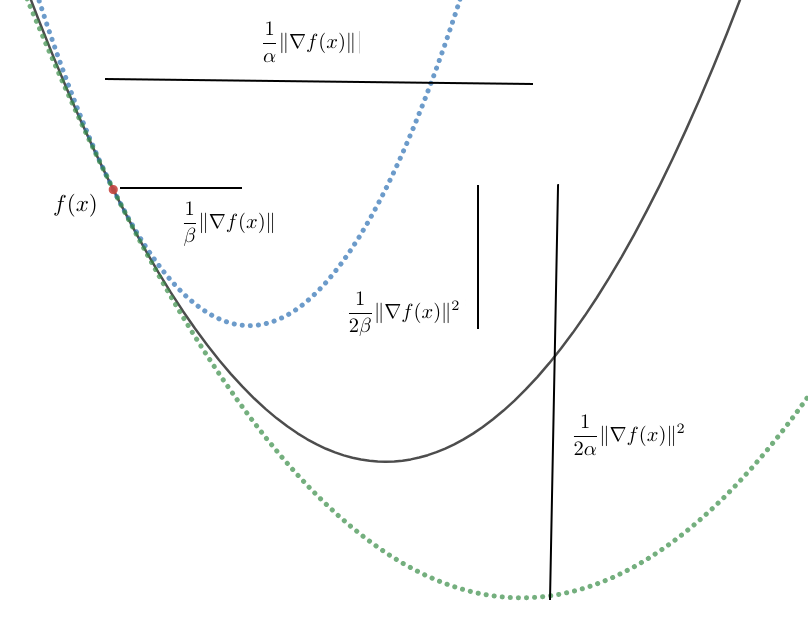
\includegraphics[width=0.5\textwidth]{img/parabolas} 
        \caption{Visualization of the smoothness bound (blue) and the strong convexity bound (green) of a function $f$ (black). }
\end{figure}

We make two important remarks about the previous analysis. Firstly, gradient descent uses the assumption of $\beta$-smoothness to guarantee maximal decrease if we move in the direction of the gradient and secondly, the decrease is better if the norm of the gradient is large. We will note later that the regret of mirror descent is lower when the norm of the gradient is low, and this along the second remark is what we can leverage to combine gradient and mirror descent. But let's focus first in the first remark. The maximal decrease on the objective we can guarantee from $x_k$ occurs when we minimize, as we did before with our toy example, the bound that is given by the $\beta$-smoothness assumption, which is
\[
    f(y) \leq f(x_k) + \langle \nabla f(x_k), y-x_k \rangle + \frac{\beta}{2} \|{y-x}\|^2,
\]
for every $y \in \X$. Note that for enough regular functions, smoothness condition can be derived by upper bounding a second order multivariate Taylor expansion using that the Hessian's eigenvalues are upper bounded by $\beta$. It is an easy way to remember the inequality. So we can define the next point as
 \begin{align}\label{general_grad_descent}
     \begin{aligned}
     x_{k+1} := &\argmin_{y \in \X} \left\{ f(x_k) + \langle \nabla f(x_k), y-x_k \rangle  +\frac{\beta}{2}\|{y-x_k}\|^2\right\} \\
    = &\argmin_{y \in \X} \left\{ \langle \nabla f(x_k), y-x_k \rangle  +\frac{\beta}{2}\|{y-x_k}\|^2\right\}.
    \end{aligned}
\end{align}
If we take $\|{\cdot}\|_2$ and $\X = \R^n$ we are searching for the minimizer in a quadratic function $a y^t y + b^t y + c $, ($a \in \R; b, c \in \R^n$) which is $-\frac{b}{2a}$ or in our case
\[
    -\frac{\nabla f(x_k) - 2 x_k \beta/2}{2 \beta/2} = x_k - \frac{1}{\beta}\nabla f(x_k).
\]
which matches our previous analysis. Maybe the following, for a general convex set $\X$, is more interesting (we subtract constant terms inside the $\argmin$'s):
\begin{align*}
    \argmin_{y \in \X} \left\{ \left\|{\left(x_k - \frac{1}{\beta}\nabla f(x_k)\right) - y}\right\|^2 \right\} \stackrel{?}{=} \argmin_{y \in \X} \left\{ \langle \nabla f(x_k), y-x_k \rangle  +\frac{\beta}{2}\|{y-x_k\|}^2\right\} \\
    \Leftrightarrow \argmin_{y \in \X} \left\{ \langle y, y\rangle - 2\left\langle y, \left(x_k - \frac{1}{\beta} \nabla f(x_k)\right)\right\rangle\right\} \stackrel{?}{=} \argmin_{y \in \X} \left\{ \langle \nabla f(x_k), y\rangle + \frac{\beta}{2}(\langle y, y\rangle - 2\langle x_k, y\rangle)\right\}. \\
\end{align*}
It is clear that the two $\argmin$'s of the last expression are the same, since we can obtain the left hand side by dividing by $\frac{\beta}{2}$ in the $\argmin$ of the right hand side. This means that our rule for projected gradient descent computes the point in $\X$ whose decrease guarantee given by the $\beta$-smoothness of $f$ is maximal among all the points in $\X$. Gradient descent for general norms is defined by rule (\ref{general_grad_descent}). We denote 

\[
    \Prog(x) := - \min_{y\in\X} \left\{ \langle \nabla f(x), y-x + \frac{\beta}{2} \|{y-x}\|^2\right\} \geq 0.
\]

By the definition of $x_{k+1}$ it is clear that $f(x_{k+1}) \leq f(x_k) - \Prog(x)$ (and $\Prog(x) = \frac{1}{2\beta} \|\nabla f(x)\|_\ast^2$ if $\X = \R^n$). We will call $\Grad(x)$ to the $\argmin$ of the previous expression.

In short, we can say that \textbf{gradient descent at each iteration maximizes the guaranteed decrease}. 

Our second remark was that with $\X = \R^n$ and $\|\cdot \|_2$ the decrease is better if $\|\nabla f(x)\|$ is larger. An intuition that we will formalize later is that mirror descent for $\X = \R^n$ and $\|\cdot \|_2$ suffers from a small loss . In general we will prove that a bound for the mirror descent loss is going to have a term easy to control and something proportional to $\Prog(x)$. So when mirror descent suffers from a large loss, gradient descent decreases the objective a lot, and when gradient descent does not have a large guaranteed decrease, mirror descent's loss will be small. This is the key idea of linear coupling, it can be used to obtain a clean accelerated method.

We saw last week that mirror descent tackles the dual optimization problem by constructing lower bounds to the optimum. Recall that each queried gradient $\nabla f(x)$ can be viewed as a hyperplane lower bounding the objective $f$, that is, $f (y) \geq f (x)+ \langle \nabla f (x), y-x \rangle$ for all $y$. Mirror-descent methods attempt to carefully construct a convex combination of these hyperplanes in order to yield even a stronger lower bound. From this point of view our claimed intuition about mirror descent having a small loss when $\|\nabla f(x)\|_2$ is small should be clear. We will denote
\[
    \Mirr(\xi) := \argmin_{y \in \X} \left\{ V_x(y) + \langle \xi, y-x \rangle \right\}.
\]
Note that a mirror descent step is $x' = \Mirr(\eta \partial f(x))$. 



\begin{figure}[h!] \label{mirror_descent_dual_loss}
\centering
        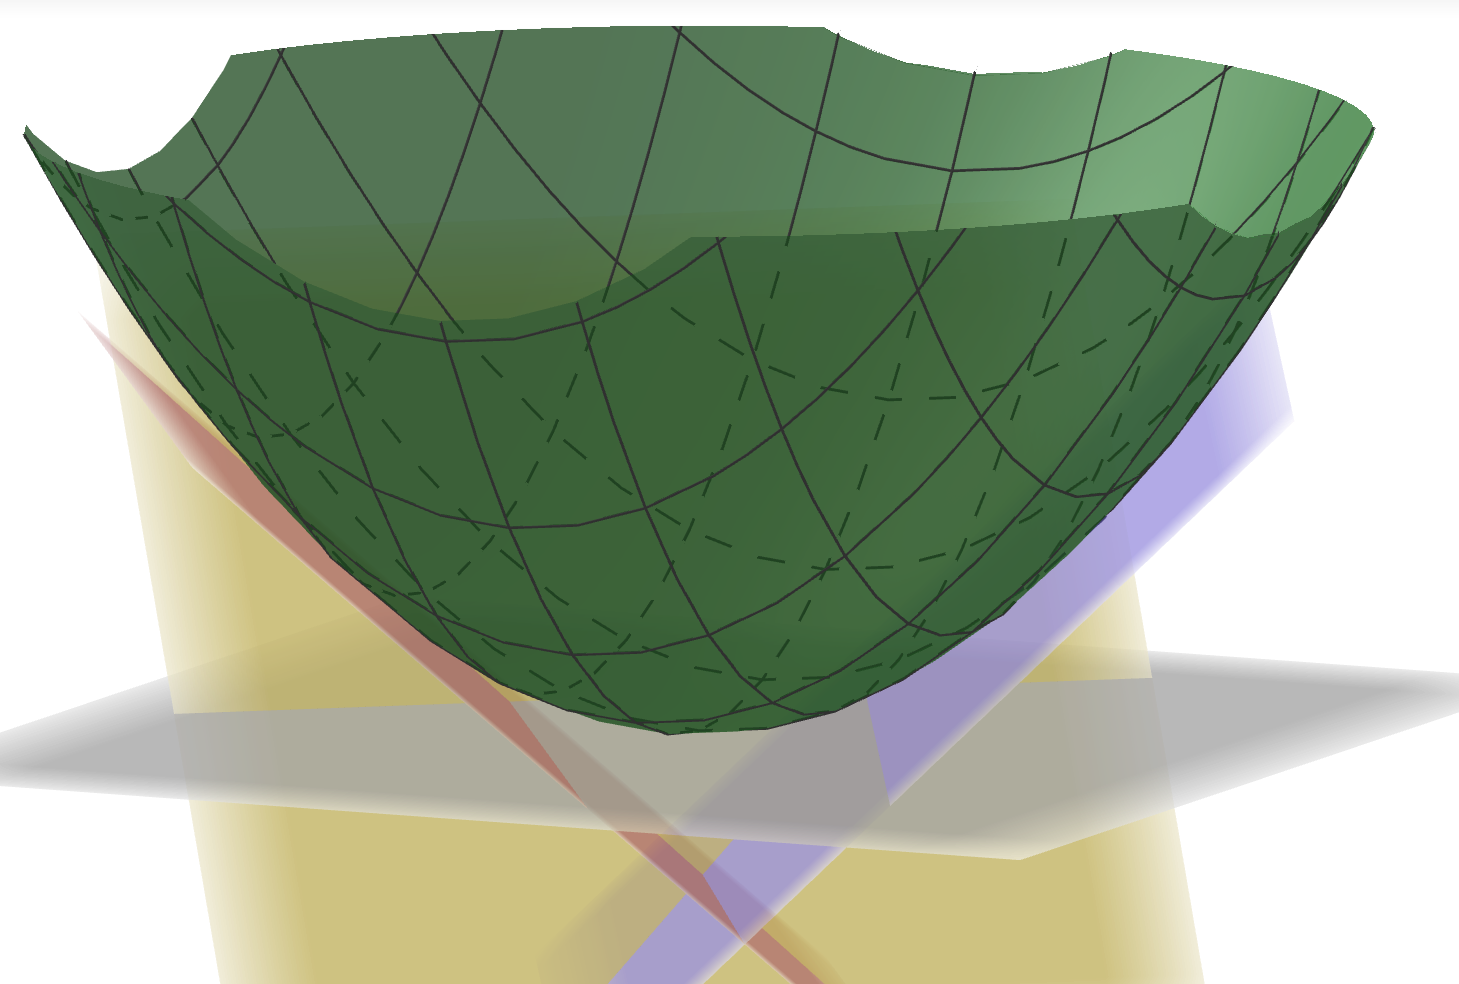
\includegraphics[width=0.5\textwidth]{img/mirror_descent_dual_loss} 
        \caption{TODO Mirror descent dual loss}
\end{figure}

It is clear that if we have several hyperplanes lower bounding the epigraph of our function we could pick a point $x$ with a small loss, that is, the difference $f(x)-f(x^\ast)$ is small. That is because the difference between the optimum and the maximum of the lower bound is small. Figure \ref{mirror_descent_dual_loss} there is a visualization of this process. In general, instead of picking the best point of the lower bound, which could need the solution of an expensive convex problem, we just take the mean of the points that we used to defined the hyperplanes and that point is good enough for the analysis. Of course this happens because mirror descent does not pick the hyperplanes naively.

%TODO mention complexity of mirror descent. We use nemirovski mirror descent, check if it is the same that it is presented in week 5
%TODO mention mirror's descent key lemma (and proof if it wasn't proved in week 5)

\textbf{Thought experiment.} For sake of demonstrating the idea, suppose $\| \nabla f(x) \|_2$, the norm of the observed gradient, is \textbf{either} always $\geq K$, or always $\geq K$, where $K$ will be determined later. Under such ``wishful assumption'', we can propose the following algorithm: the norm of the gradient is always $\geq K$ perform $T$ gradient descent steps. Otherwise perform $T$ mirror descent steps. To analyze such an algorithm, suppose without loss of generality we start with some point $x_0$ whose objective distance $f(x_0 )-f(x^\ast )$ is at most $2\epsilon$, and we want to find some $x$ so that

If $T$ gradient descent steps are performed, the objective decreases by at least $\frac{\|\nabla f(\cdot)\|_2^2}{2L} \geq \frac{K^2}{2L}$ per step and we only need $T \geq \Omega\left(\frac{\epsilon L}{K^2}\right)$ steps to achieve an $\epsilon$ accuracy. If $T$ mirror descent steps are performed, we need $T \geq \Omega\left(\frac{K^2}{\epsilon^2}\right)$ steps according to the mirror descent convergence. In sum, we need $T \geq \Omega\left( \max \left\{ \frac{\epsilon L}{K^2}, \frac{K^2}{\epsilon^2}\right\}\right)$ steps to converge to an $\epsilon$-minimizer. Setting K to be the magic number to balance the two terms, we only need $T \geq \Omega\left( \sqrt{\frac{L}{\epsilon}}\right)$ iterations. This means that in the general case in which $f(x_0) - f(x^\ast) \leq d $ we only need $T \geq \Omega \left(\sqrt{\frac{L}{\epsilon}}\left(\frac{\epsilon}{d} + \frac{2\epsilon}{d} + \dots + \frac{1}{2} + 1 \right)\right) = \Omega \left( \sqrt{\frac{L}{\epsilon}}\right)$.
%TODO fix \epsilon/d

\subsection{Warm-Up Method with Fixed Step Length}
The key ideas of this method will be the same as the ones for the final method, but we start with this simpler method for simplicity. As we mentioned previously, at each iteration linear coupling performs a gradient descent step and a mirror descent and the point for the next iteration is a convex combination of the points obtained by gradient and mirror descent. The key of the proof is to see that the loss in which mirror descent incurs is something proportional to the gradient descent guaranteed decrease (plus a couple of Bregman divergences that will telescope) and using this fact to see that a particular convex combination of mirror and gradient descent incurs in a similar loss.

Formally, we start with $x_0 = y_0 = z_0$. In each iteration $k= 0, 1, \dots, T-1$ we define $x_{k+1} \gets \tau z_k + (1-\tau) y_k$ and then we perform:
\begin{itemize}
    \item A gradient step $y_{k+1} \gets \Grad(x_{k+1})$.
    \item A mirror step $z_{k+1} \gets \Mirr\left(\eta \nabla f(x_{k+1})\right)$.
\end{itemize}
The choices of $\eta$ and $\tau$ will become clear at the end of this section,, but from a high level $\eta$ is determined by the mirror descent analysis, similarly to what we saw last week, and $\tau$ will be determined as the best parameter to balance gradient and mirror descent, similar to $K$ in the previous thought experiment.

The two key ideas mentioned before materialized in the following two lemmas:
\begin{lemma}\label{lemma:mirror_bound}
    For every $u \in \X = \R^n$,
    \begin{align}\label{mirror_bound_in_linear_coupling}
        \begin{aligned}
            \eta \langle \nabla f(x_{k+1}), z_k -u \rangle & \leq \frac{\eta^2}{2} \| \nabla f(x_{k+1})\|^2_\ast + V_{z_k}(u) - V_{z_{k+1}}(u) \\
                                                       & \leq \eta^2 \beta (f(x_{k+1}) - f(y_{k+1})) + V_{z_k}(u) - V_{z_{k+1}}(u). \\
        \end{aligned}
    \end{align}
\end{lemma}

\begin{proof}
    The first inequality is Lemma \ref{todo}, in which the mirror descent analysis is based. The second inequality is from the gradient step guarantee $f(x_{k+1}) - f(y_{k+1}) \geq \frac{1}{2L}\| \nabla f(x_{k+1})\|^2_\ast$.
\end{proof}

The second lemma bounds the actual regret at $x_{k+1}$ and picks $\tau$ so that we can telescope the sum of the regrets.

\begin{lemma}\label{lemma_simplified_coupling}[Coupling] Letting $\tau \in (0, 1)$ satisfy that $\frac{1-\tau}{\tau}  \eta\beta$, we have that
\[
    \forall u \in \X = \R^n, \quad \eta \langle \nabla f(x_{k+1}), x_{k+1} - u \rangle \leq \eta^2\beta\left( f(y_k) - f(y_{k+1})\right)a + \left( V_{z_k} - V_{z_{k+1}}(u)\right).
\]
\end{lemma}

\begin{proof}
    We can compute easily the difference between the regrets at $x_{k+1}$ and at $z_k$ using the definition of $x_{k+1}$.
    \begin{align}\label{actual_regret_simplified_linear_coupling}
        \begin{aligned}
            \eta \langle \nabla f(x_{k+1}), x_{k+1} - u \rangle - \eta \langle \nabla f(x_{k+1}), z_k - u \rangle = \eta \langle \nabla f(x_{k+1}), x_{k+1} - z_k \rangle  \\
            = \frac{(1-\tau)\eta}{\tau} \langle \nabla f(x_{k+1}), y_k - x_{k+1} \rangle \leq \frac{(1-\tau)\eta}{\tau} (f(y_k) - f(x_{k+1})).
        \end{aligned}
    \end{align}
    Above, we used the fact that $\tau(x_{k+1} - z_k) = (1-\tau)(y_k -x_{k+1})$, as well as the convexity of $f$. It is immediate that by choosing $\frac{1-\tau}{\tau} = \eta \beta$ and combining \ref{mirror_bound_in_linear_coupling} and \ref{actual_regret_simplified_linear_coupling} we have the result.
\end{proof}

If we telescope \ref{lemma_simplified_coupling} for $k= 0, 1, \dots, T-1$ and setting $\bar{x} := \frac{1}{T} \sum_{k=0}^{T-1} x_k$  and $u = x^\ast$, we have
\begin{equation}\label{final_lemma_simplified_coupling}
    \eta T \left( f(\bar{x}) - f(x^\ast) \right)\leq \sum_{k=0}^{T-1} \eta \langle \nabla f(x_k), x_k - x^\ast \rangle \leq \eta^2 \beta \left( f(y_0) - f(y_T) \right) + V_{x_0} - V_{x_T}(x^\ast).
\end{equation}

Suppose our initial point is of error at most $d$, that is $f (y_0 ) − f (x^\ast ) \leq d$, and suppose $V_{x_0}(x^\ast) \leq \Theta$, then \ref{final_lemma_simplified_coupling} gives $f (\bar{x})-f (x^\ast ) \leq \frac{1}{T}\left( \eta \beta d + \Theta/\eta\right)$. Choosing $\eta = \sqrt{\Theta/(\beta d)}$ to be the value that balances the above two terms (it is essentially the same way of choosing $\eta$ in mirror descent), we obtain that $f (x) − f (x^\ast ) \leq \frac{\sqrt{\beta \Theta d}}{T}$. In other words, in $T = 4 \sqrt{\beta\Theta/d}$ steps, we can obtain some $\bar{x}$ satisfying $f (\bar{x}) − f (x^\ast ) \leq d/2$, halving the distance to the optimum. If we restart this entire entire procedure a few number of times, halving the distance for every run, then we obtain an $\epsilon$-approximate solution in
\[
    T = O \left(\sqrt{\beta \Theta / \epsilon} + \sqrt{\beta \Theta / 2\epsilon} + \sqrt{\beta \Theta / 4 \epsilon} + \dots \right) = O\left(\sqrt{L\Theta / \epsilon}  \right)
\]
iterations. The value of $\eta = \sqrt{\Theta/(\beta d)}$ increases as time goes and therefore $\tau = \frac{1}{\eta \beta +1}$ decreases as time goes. This tells us that gradient descent is given more weight the mirror step when we are close to the minimum.  This fact can be counter-intuitive because when it is closer to the optimum, the observed gradients will become smaller, and therefore mirror steps should perform well according to the thought experiment. This understanding is incorrect, when it is closer to the optimum, the threshold between large and small gradients also becomes smaller, so one cannot rely only on mirror steps.

\subsection{Final Method with Variable Step Lengths}
This final method will change $\eta$ and $\tau$ gradually to obtain an algorithm that does not need to know the bounds $\Theta$ and $d$. This approach will also work for any convex restriction set $\X$. The final algorithm is the following:

\begin{algorithm}[H]\label{alg:AGM}
\scriptsize
\caption{AGM $(f, w, x_0, T)$}
   \label{alg:AGM}
   \begin{algorithmic}[1]
   \REQUIRE $f$ a differentiable and convex function on $\X$ that is $\beta$-smooth with respect to $\|\cdot\|$, $w$ the $DGF$ function that is $1$-strongly convex with respect to the same $\|\cdot\|$ over $\X$. $x_0$ some initial point and $T$ the number of iterations.
   \ENSURE $y_T$ such that $f(y_T) -f(x^\ast) \leq \frac{4\Theta \beta}{T^2}$.
   \STATE $V_x(y) := w(y) - \langle \nabla w(x), y-x\rangle - w(x).$
   \STATE $y_0 \gets x_0, \quad z_0 \gets x_0$.
   \FOR{$ k \gets 0 $ to $T-1$}
       \STATE $\eta_{k+1} \gets \frac{k+2}{2\beta}$, and $\tau_k \gets \frac{1}{\eta_{k+1}\beta} = \frac{2}{k+2}$
       \STATE $x_{k+1} \gets \tau_k z_k + (1-\tau_k)y_k$.
       \STATE {$y_{k+1} \gets \Grad(x_{k+1})$ \hfill\hfill $\left( := \argmin_{y\in\X} \left\{ \frac{\beta}{2} \| y-x_{k+1}\|^2 + \langle \nabla f(x_{k+1}), y-x_{k+1} \rangle \right\}\right) $}
       \STATE{ $z_{k+1} \gets \Mirr_{z_k}\left(\eta_{k+1} \nabla f (x_{k+1})\right)$ \hfill\hfill $\left( := \argmin_{y\in\X} \left\{ V_{z_k}(z) + \langle \eta_{k+1} \nabla f(x_{k+1}), z-z_k \rangle \right\}\right) $}

   \ENDFOR
   \STATE {\bfseries return} $y_T$
\end{algorithmic}
\end{algorithm}

We will prove that this method is accelerated. In particular, we have the following theorem.

\begin{theorem}\label{thm:linear_coupling}
    If $f(x)$ is $\beta$-smooth w.r.t. $\|\cdot\|$ on $\X$, and $w(x)$ is $1$-strongly convex w.r.t. $\|\cdot\|$ on $\X$, then Algorithm \ref{alg:AGM} outputs $y_t$ satisfying $f(y_T) - f(x^\ast) \leq 4 \Theta \beta /T^2$, where $\Theta$ is any upper bound on $v_{x_0}(x^\ast)$.
\end{theorem}

We will use two lemmas, that are the analogous to Lemma \ref{lemma:mirror_bound} and Lemma \ref{lemma_simplified_coupling}, that we will prove after the proof of the theorem.

\begin{lemma}\label{lemma:mirror_bound_general}
    If $\tau_k = \frac{1}{\eta_{k+1}\beta}$, then linear coupling satisfies that for every $u \in \X$,
    \begin{align*}\label{actual_regret_linear_coupling}
        \begin{aligned}
            \eta \langle \nabla f(x_{k+1}), x_{k+1} - u \rangle &\leq \eta^2\beta \Prog(x_{k+1}) + \left( V_{z_k} - V_{z_{k+1}}(u)\right) \\
                                                                &\leq \eta_{k+1}^2 \left( f(x_{k+1}) - f(y_{k+1})\right) + \left( V_{z_k} - V_{z_{k+1}}(u)\right).
        \end{aligned}
    \end{align*}
\end{lemma}

\begin{lemma}[Coupling]\label{lemma:coupling} For any $u\in\X$,
    \[
        \left(\eta_{k+1}^2 \beta \right) f(y_{k+1}) - \left( \eta^2_{k+1} \beta - \eta_{k+1}\right)f(y_k) + \left( V_{z_{k+1}} - V_{z_k}\right) \leq \eta_{k+1} f(u).
    \]
\end{lemma}

\begin{proof}[Proof of Theorem \ref{thm:linear_coupling}]
    In order to telescope Lemma \ref{lemma:coupling} we only need to set the sequence of $\eta_k$ so that $\eta_k^2 \beta \approx \eta_{k+1}^2 \beta - \eta_{k+1}$ as well as $\tau_k = 1/\eta_{k+1}\beta \in (0, 1]$. In Algorithm \ref{alg:AGM} $\eta_k =  \frac{k+1}{2\beta}$ so that $\eta_k^2 = \eta^2_{k+1} -\alpha_{k+1} + \frac{1}{4\beta}$. Summing up Lemma \ref{lemma:coupling} for $k = 0, 1, \dots, T-1$, we obtain
\[
    \eta^2_T \beta f(y_T) + \sum_{k=1}^{T-1}\frac{1}{4\beta} + \left( V_{x_T}(u) - V_{z_0}(u)\right) \leq   \sum_{k=1}^T \eta_k f(u).
\]
By choosing $u= x^\ast$, we notice that $\sum_{k=1}^T \eta_k = \frac{T(T+3)}{4\beta}$, $f(y_t) \geq f(x^\ast)$, $V_{z_T} \geq 0$ and $V_{z_0} (x^\ast) \leq \Theta$. Therefore, we obtain
\[
    \frac{(T+1)^2}{4\beta^2}\beta f(y_T) \leq \left(  \frac{T(T+3)}{4L} - \frac{T-1}{4L}\right)f(x^\ast) + \Theta,
\]
which after simplification implies $f(y_T)\leq f(x^\ast) + \frac{4\Theta \beta}{(T+1)^2}$.
\end{proof}


\begin{proof}[Proof of Lemma \ref{lemma:mirror_bound_general}]
    The second inequality of the lemma is again by the gradient descent guarantee $f(x_{k+1}) - f(y_{k+1})) \geq \Prog(x_{k+1})$. To prove the first one, we first write down the key inequality of mirror-descent analysis. 
\begin{align*}\label{actual_regret_linear_coupling}
    \begin{aligned}
        \eta_{k+1} \langle \nabla f(x_{k+1}), z_{k} - u \rangle &= \langle \eta_{k+1} \nabla f(x_{k+1}), z_k - z_{k+1} \rangle + \langle \eta_{k+1} \nabla f(x_{k+1}), z_{k+1} - u \rangle \\
                                                                &\leq  \langle \eta_{k+1} \nabla f(x_{k+1}), z_k - z_{k+1} \rangle + \langle -\nabla V_{z_k}(u), z_{k+1} - u \rangle \\
                                                                &=  \langle \eta_{k+1} \nabla f(x_{k+1}), z_k - z_{k+1} \rangle + V_{z_k}(u) - V_{z_{k+1}}(u) + V_{z_k}(z_{k+1}) \\
                                                                &\leq  \left( \langle \eta_{k+1} \nabla f(x_{k+1}), z_k - z_{k+1} \rangle - \frac{1}{2}\|z_k - z_{k+1}\|^2 \right)  +  \left( V_{z_k}(u) - V_{z_{k+1}}(u) \right) \\
    \end{aligned}
\end{align*}
The first inequality is due to the minimality of $z_{k+1} = \argmin_{z\in\X} \{V_{z_k} + \langle \eta_{k+1} \nabla f(x_{k+1}), z \rangle\}$, which implies that  $\langle \nabla V_{z_k} (z_{k+1}) + \eta_{k+1} \nabla f(x_{k+1}), u-z_{k+1} \rangle \geq 0 $ for all $u \in \X$. The second inequality is because $V_x(y) \geq \frac{1}{2} \|x-y\|^2$ by the strong convexity of the $w(\cdot)$. If we apply Cauchy-Shwartz to the first summand of the last expression above and the fact that $az-bz^2 \leq \frac{a^2}{4b}, \ \forall z \in \R$ we get
\[
    \left( \langle \eta_{k+1} \nabla f(x_{k+1}), z_k - z_{k+1} \rangle - \frac{1}{2}\|z_k - z_{k+1}\|^2 \right) \leq \left(\eta_{k+1}\|\nabla f(x_{k+1})\|_\ast \right) \|z_k - z_{k+1}\| - \frac{1}{2}\|z_k - z_{k+1}\|^2 \leq \frac{\eta_{k+1}^2}{2} \|\nabla f(x_{k+1})\|_\ast^2
\]
and thus we have the result for $\X = \R^n$. For the general constrained we need to use the special choice of $\tau_k = 1/\eta_{k+1} \beta$ as follows. Letting $v:= \tau_k z_{k+1} + (1-\tau_K) y_k \in \X$ so that $x_{k+1} - v = (\tau_k z_k + (1-\tau_k)y_k) -v = \tau_k(z_k-z_{k+1})$, we have
\begin{align*}\label{actual_regret_linear_coupling}
    \begin{aligned}
        &\langle \eta_{k+1} \nabla f(x_{k+1}), z_k - z_{k+1} \rangle - \frac{1}{2}\|z_k - z_{k+1}\|^2  \\
        = & \left\langle \frac{\eta_{k+1}}{\tau_k} \nabla f(x_{k+1}), x_{k+1} - v \right\rangle - \frac{1}{2\tau_k^2} \|x_{k+1} - v \|^2 \\
        = & \eta_{k+1}^2 \beta \left( \langle \nabla f(x_{k+1}), x_{k+1} -v \rangle - \frac{\beta}{2} \|x_{k+1} - v\|^2\right) \leq \eta_{k+1}^2 \beta \Prog(x_{k+1})
    \end{aligned}
\end{align*}
where the last inequality is from the definition of $\Prog(x_{k+1})$.

\end{proof}


\begin{proof}[Proof of Lemma \ref{lemma:coupling}]
We can derive the lemma from the following inequalities
\begin{align*}\label{actual_regret_linear_coupling}
    \begin{aligned}
        &\ \eta_{k+1}(f(x_{k+1}) -f(u)) \\
        \leq &\ \eta_{k+1} \langle \nabla f(x_{k+1}), x_{k+1} -u \rangle \\
        = &\ \eta_{k+1} \langle \nabla f(x_{k+1}), x_{k+1} -z_{k} \rangle + \eta_{k+1} \langle \nabla f(x_{k+1}), z_k -u \rangle \\
        = &\ \frac{(1-\tau_k)\eta_{k+1}}{\tau_k} \langle \nabla f(x_{k+1}), y_k - x_{k+1} \rangle + \langle \nabla f(x_{k+1}), z_k - u \rangle \\
        \leq &\ \frac{(1-\tau_k)\eta_{k+1}}{\tau_k}(f(y_k)-f(x_{k+1})) + \eta_{k+1} \langle \nabla f(x_{k+1}), z_k-u \rangle \\
        \leq &\ \frac{(1-\tau_k)\eta_{k+1}}{\tau_k}(f(y_k)-f(x_{k+1})) + \eta_{k+1}^2 \beta (f(x_{k+1}) - f(y_{k+1}))  + V_{z_k}(u) - V_{z_{k+1}}(u)\\
        = &\ (\eta_{k+1}^2\beta -\eta_{k+1})f(y_k) -(\eta_{k+1}^2 \beta)f(y_{k+1})  +\eta_{k+1}f(x_{k+1})   + \left( V_{z_k}(u) - V_{z_{k+1}}(u)\right)\\
    \end{aligned}
\end{align*}
where the lines $4,5,6$ and $7$ are obtained, respectively, by $(4)$ the choice of $x_{k+1}$ that satisfies $\tau_k(x_{k+1} - z_k) = (1-\tau_k) (y_k - x_{k+1})$; $(5)$ is by the convexity of $f$ and $1-\tau_k \geq 0$; $(6)$ uses Lemma \ref{lemma:mirror_bound_general} and $(7)$ uses the choice of $\tau_k = 1/\alpha_{k+1}\beta$.
\end{proof}
